% Preview source code

%% LyX 2.1.4 created this file.  For more info, see http://www.lyx.org/.
%% Do not edit unless you really know what you are doing.
\documentclass[12pt,english]{article}
\renewcommand{\familydefault}{\sfdefault}
\usepackage[T1]{fontenc}
\usepackage[latin9]{inputenc}
\usepackage[a4paper]{geometry}
\geometry{verbose,tmargin=25mm,bmargin=25mm,lmargin=25mm,rmargin=25mm}
\usepackage{fancyhdr}
\pagestyle{fancy}
\usepackage{color}
\usepackage{amstext}
\PassOptionsToPackage{normalem}{ulem}
\usepackage{ulem}

\makeatletter
%%%%%%%%%%%%%%%%%%%%%%%%%%%%%% User specified LaTeX commands.
\usepackage{titling, graphicx}
\usepackage{tikz}

\usetikzlibrary{shapes,arrows.meta, intersections, graphs, graphs.standard}
\usetikzlibrary{math}

\date{}
%\setlength\parindent{0pt}

\pretitle{\begin{center} \Large \bf \vspace{-2em}}
\posttitle{\par\end{center}\vspace{-1.5em}}
\preauthor{\begin{center} \large \lineskip 1em \begin{tabular}[t]{c}}
\postauthor{\end{tabular}\par\end{center}\vspace{-5em}}

\rhead{Dr. Erku\c{s}}
\lhead{\thetitle}

\fancypagestyle{firststyle}
{
\lhead{Istanbul Technical University}
\chead{\includegraphics[width=0.75cm, keepaspectratio=true]{logo.pdf}}
\rhead{Civil Engineering Department}
}

\makeatother

\usepackage{babel}
\begin{document}

\title{YAP 618 \textendash{} Homework Assignment 2}


\author{Dr. Bar\i \c{s} Erku\c{s}}

\maketitle
\thispagestyle{firststyle}


\section{Numerical Solution of Equations of Motion}


\subsection{SDOF Systems}

Consider the single-degree-of-freedom (SDOF) system shown below. Develop
a \textsc{Matlab} code that reads a text file of ground motion acceleration
data of an historical earthquake and solves the equation of motion.
The program should find and plot $x(t)$, $\dot{x}(t)$, $\ddot{x}(t)$,
inertia force and forces generated by stiffness and damping. Solve
a sample system using the program written and program NONLIN for the
same ground acceleration. Compare the results. \textcolor{blue}{(Due
4 March 2016, 5:00pm)}

\begin{center}
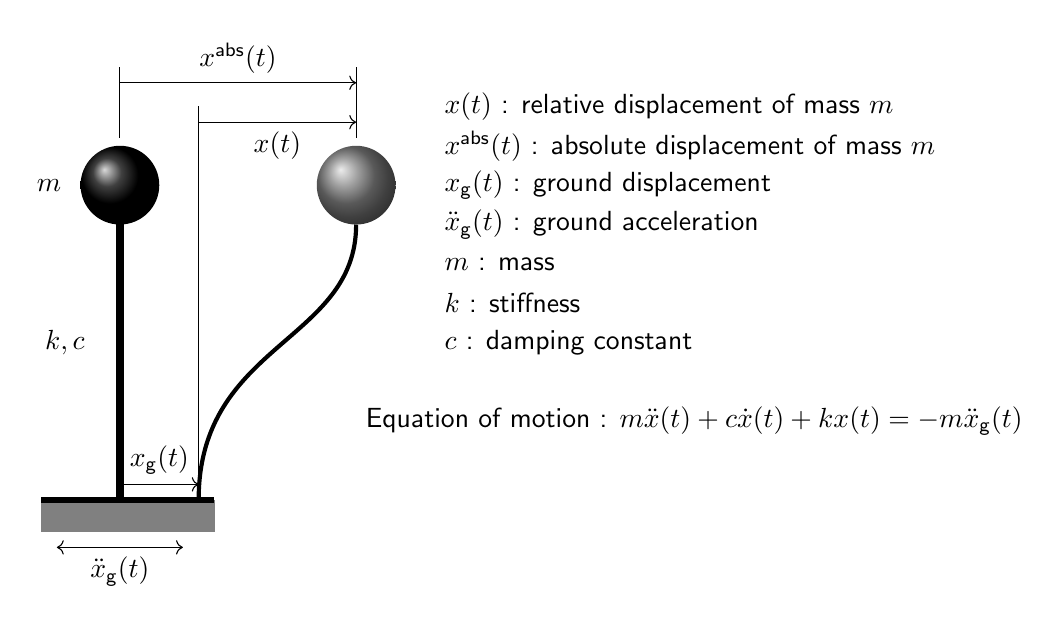
\begin{tikzpicture} [scale=1]
 \draw [line width=0pt, color = white] (0, 6);
 \draw [line width = 3pt] (0,0) -- (0,4);
 \shade [ball color=black] (0,4) circle [radius = 0.5cm];
 \draw [line width=1.5pt] (1,0) .. controls (1,2) and (3,2) .. (3,3.5);
 \shade [ball color=gray] (3,4) circle [radius = 0.5cm];
 \draw (0, 4.6) -- (0, 5.5);
 \draw (3, 4.6) -- (3, 5.5);
 \draw [->](0, 5.3) -- (3, 5.3);
 \draw (1.5, 5.3) node[anchor=south] {$x^{\mbox{\scriptsize{abs}}}(t)$};
 \draw (1,0.1) -- (1,5.0);
 \draw [->] (1,4.8) -- (3,4.8);
 \draw (2, 4.8) node[anchor=north] {$x(t)$};
 \filldraw [gray] (-1,-0.4) rectangle (1.2, 0);
 \draw [line width=2pt] (-1,0) -- (1.2,0);
 \draw (-0.9cm, 4cm) node {$m$};
 \draw (-0.7cm, 2cm) node {$k, c$};
 \draw [->] (0,0.2) -- (1,0.2);
 \draw (0.5, 0.2) node[anchor=south] {${x}_{\mbox{\scriptsize{g}}}(t)$};
 \draw [<->] (-0.8,-0.6) -- (0.8,-0.6);
 \draw (0,-0.6) node[anchor=north] {$\ddot{x}_{\mbox{\scriptsize{g}}}(t)$};
 \draw (4,5)   node[anchor=west] {$x(t)$ : relative displacement of mass $m$};
 \draw (4,4.5) node[anchor=west] {$x^{\mbox{\scriptsize{abs}}}(t)$ : absolute displacement of mass $m$};
 \draw (4,4.0) node[anchor=west] {${x}_{\mbox{\scriptsize{g}}}(t)$ : ground displacement};
 \draw (4,3.5) node[anchor=west] {$\ddot{x}_{\mbox{\scriptsize{g}}}(t)$ : ground acceleration};
 \draw (4,3)   node[anchor=west] {$m$ : mass};
 \draw (4,2.5) node[anchor=west] {$k$ : stiffness}; 
 \draw (4,2)   node[anchor=west] {$c$ : damping constant};
 \draw (3,1)   node[anchor=west] {Equation of motion : $m\ddot{x}(t) + c\dot{x}(t) + kx(t) = -m\ddot{x}_{\mbox{\scriptsize{g}}}(t)$};
\end{tikzpicture}
\par\end{center}


\subsection{MDOF Systems}

Consider the general form of equation of motion for a multi-degree-of-freedom
(MDOF) system given below:

\begin{center}
$\mathbf{M}\ddot{\mathbf{x}}(t)+\mathbf{C}\dot{\mathbf{x}}(t)+\mathbf{K}\mathbf{x}(t)=-\mathbf{M}\mathbf{r}\mathbf{a}_{\textrm{g}}(t)$
\par\end{center}

\noindent where $\mathbf{M}$, $\mathbf{C}$, $\mathbf{K}$ are mass,
damping, and stiffness matrices; $\ddot{\mathbf{x}}(t)$, $\mathbf{\dot{x}}(t)$
and $\mathbf{x}(t)$ are acceleration, velocity and displacement vectors
and $\mathbf{a}_{\textrm{g}}(t)$ is the ground acceleration vector.
Develop a \textsc{Matlab} code that solves the equation of motion
for given system matrices, $\mathbf{M}$, $\mathbf{C}$, $\mathbf{K}$
and $\mathbf{r}$, and given ground acceleration data, $\mathbf{a}_{\textrm{g}}(t)$.
Consider that ground accelearation vector has horizontal and vertical
components, $\mathbf{a}_{\textrm{g}}(t)=\left[\begin{array}{cc}
\mathbf{a}_{\textrm{g,X}}(t), & \mathbf{a}_{\textrm{g,Y}}(t)\end{array}\right]^{\textrm{T}}$. The code should plot $\ddot{\mathbf{x}}(t)$, $\mathbf{\dot{x}}(t)$
and $\mathbf{x}(t)$ for given degrees of fredoom. \textcolor{blue}{(Due
11 March 2016, 5:00pm)}


\section{Derivation of Equation of Motion for Frames}

Consider a general frame as shown below. Develop an algorithm that
can derive the mass and stiffness matrices ($\mathbf{M}$, and $\mathbf{K}$)
that will appear in the equation of motion of the structure. Consider
that ground accelearation vector has horizontal and vertical components,
$\mathbf{a}_{\textrm{g}}(t)=\left[\begin{array}{cc}
a_{\textrm{g,X}}(t), & a_{\textrm{g,Y}}(t)\end{array}\right]^{\textrm{T}}$. The algorithm \uline{does not need to be} in \textsc{Matlab}
m-file syntax.

\begin{center}
\tikzmath{
int \ns, \nb, \ncol, \nlev, \i, \j;
real \sh, \bw, \startx, \starty, \xx, \y;
real \supw, \suph;
coordinate \c;
\ns = 3; %number of storys
\nb = 3; %number of bays
\ncol = \nb+1; %number of columns
\nlev = \ns+1; %number of levels
\sh = 2; %story height
\bw = 2.5; % bay width
\starty = 0; %starting coordinate y
\startx = 0; %starting coordinate x
\supw = 1; %support width
\suph = 0.3; %support height
for \i in {1,...,{\nlev}}{
\y{\i} = \starty + (\i-1)*\sh;
for \j in {1,...,{\ncol}}{
\x{\j} = \startx + (\j-1)*\bw;
};
};
}
\begin{tikzpicture} [scale=1]
\draw [line width=0pt, color = white] (0, \y{\nlev}+2);
\foreach \i in {2,...,{\nlev}}
{
\draw [line width = 1pt] (\x{1},\y{\i}) -- (\x{\ncol},\y{\i});
}
\foreach \j in {1,...,{\ncol}}
{
\draw [line width = 1pt] (\x{\j},\y{1}) -- (\x{\j},\y{\nlev});
}
\draw [{->}] (\x{\ncol}+\supw,\y{1}) -- +(1,0) node[anchor=west]{$X$};
\draw [{->}] (\x{1},\y{\nlev}+0.5) -- +(0,1) node[anchor=east]{$Y$};
\foreach \j in {1,...,{\ncol}}
{
\filldraw [gray] (\x{\j},\y{1}) +({-\supw/2},-\suph) rectangle +({\supw/2},\y{1});
\draw [line width = 2pt] (\x{\j},\y{1}) +({-\supw/2},\y{1}) -- +({\supw/2},\y{1});
}

\end{tikzpicture}
\par\end{center}


\subsubsection*{Hints:}
\begin{enumerate}
\item Assume that displacements of the restrained degrees-of-freedom will
be the corresponding ground displacements. For example, for a fixed
support, absolute global displacement vector will be $\mathbf{D_{\textrm{abs}}}(t)=\left[\begin{array}{ccc}
x_{\textrm{g,X}}(t), & x_{\textrm{g,Y}}(t), & 0\end{array}\right]^{\textrm{T}}$, where $x_{\textrm{g,X}}(t)$ and $x_{\textrm{g,Y}}(t)$ are the
ground displacements in the $X-$ and $Y-$directions respectively
$x^{'}$.
\item Assume that displacements of the unrestrained degrees-of-freedom will
be the summation of the displacements relative to the ground and corresponding
ground displacements. For example for a fully unrestrained joint $i$,
the displacement vector will be $\mathbf{D_{\textrm{abs}}}(t)=\left[\begin{array}{ccc}
X{}_{i}+x_{\textrm{g,X}}(t), & Y{}_{i}+x_{\textrm{g,Y}}(t), & \theta{}_{i}\end{array}\right]^{\textrm{T}}$, where $X_{i}$ and $Y_{i}$ are the global degrees-of-freedom in
the $X-$ and $Y-$directions, and $\theta{}_{i}$ is the rotational
degree-of-freedom of joint $i$.
\item Assume that there are no external static forces applied to the structure.
\item Consider that mass of structure is lumped at the joints. For the sake
of this problem assume that all frame elemants has a mass per length,
$\bar{m}$ (\textit{i}.\textit{e}., total mass of a frame element
with length $L$ is $\bar{m}L$.
\item For the components of the mass matrix that correspond to the rotational
degrees-of-freedom, you can either use the mass value that corresponds
to the translational degrees-of-freedom or a consistent mass value
(derivation of mass matrices are generally well-explained in structural
dynamics books, \textit{see e.g.} the book by Clough and Penzien)
\end{enumerate}
\textcolor{blue}{(Due 4 March 2016, 5:00pm)}
\end{document}
